% !TeX spellcheck = en_GB
% !TeX spellcheck = en_US 
\chapter{Acquisition and calibration methods.}


In order to use the above setup with the  MIR and NIR laser parameters, the methods used in this experiment are explained in this section, from the VMI calibrartion thecniques to the data analisis ands post software analiosis process. All experimental techniques were used to investigate both helium and neon clusters. 


In contrast to other spectroscopic experiments, the  Photoelectric spectra (PES) of the $e-$ VMI, looks different for each event. We assume it happend because of the size distribution of the clusters and the different intensities each cluster is exposed to, comparing the small size of the cluster compared to the laser focus. Nevertheless, the images and therefore the PES look rather similar in shape for the small clusters. For larger clusters ($<N>= 10^{6}$) different shapes show up, as show in the results section. For example some images show blops compleates uniform while others signal, shoe ghiegh intensities in the edges and lower in the centewr, like a "donut" shape as we will refeer from now.

When recording single events with both, the TOF and the VMI spectrometer, it would be desirable if both spectra could be matched and lead back to the same event. A method is described in the following section.
The disadvantage of this method is, that the maximum acquisition rate is maximum 30Hz, which is the speed of the camera. Depending on the hard drive, that is used the acquisition rate can drop to 10Hz. Furthermore, the single shot method needs low even trates of less then $10\%$. In total it results in an event rate of less then 1Hz.

\begin{figure}[hbtp]
\caption{Example images of MIr Vmi signal. On the left, a uniform blop, on the rigth a "donut " shape signal with high density signal on the borders of the edges. }
\centering
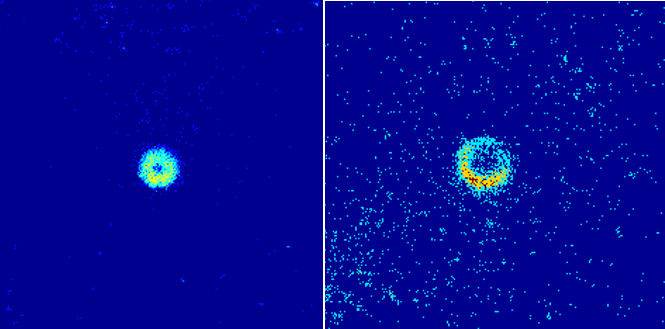
\includegraphics[scale=1]{../Images/vmi_examples.png}
\label{fig:vmiexample}
\end{figure}



\section{Camera and trigger protocol}

One of the main goal of this research, is to achieve individual data for single shots nanoplasma explosion in the VMI and TOF. The advantage, is the ability of the threat the data in a separate way to reduce the background and achieve  properties on the coulomb explosion that are not possible when data is averaged.

Two methods were developed for this work. A first approach was done using a software trigger for the CCD camera and the oscilloscope for the TOF, an Acqiris Card CC103. Using LabView, an external clock (a RasberryPi 3) was triggered by the laser, the beginning of the explosion,  at the same time, it software-trigger the camera and oscilloscope programs to start the acquisition. Having all the data acquired in the same software would allow to sort the data online and reduce the storage needed for the experiment. The Labview program was tested unsuccessfully for the data acquisition rate needed in ELI $100KHz$, the main problem was, that when a software-triggering scheme is used,  extra delays are applied due to the operating system and the communication protocols, so even the data were acquired at the same time the delays in at saving  it in the hard drive made impossible to correlate the signals.

Based on that same idea, a second approach was used. As alternative of the software triggering a hardware triggering was used. The laser triggers a delay generator that at the same time triggers the oscilloscope, a $R.S$ RTO2000 with bandwidth of 600MHZ to 6GHz,  and the camera. Two facts had to be taken into account, first, the minimal exposure time of the camera is $34\mu s$. Second, the timing between the camera receiving the trigger and the real start of the acquisition is not negligible as it is for the oscilloscope. The camera took between $5-6 \mu s$ to start after the trigger was sent. To solve this problem the triggering scheme in fig \ref{fig:triggers}.
\begin{table}[]
\label{tab:delaystriger}
\centering
\begin{tabular}{ll}
\multicolumn{2}{c}{List delays}                                          \\ \hline
\multicolumn{1}{|l|}{Channel} & \multicolumn{1}{l|}{Set to:}    \\ \hline
\multicolumn{1}{|l|}{A}                & \multicolumn{1}{l|}{$=T+0$}       \\ \hline
\multicolumn{1}{|l|}{B}                & \multicolumn{1}{l|}{$=T+1\mu s$}     \\ \hline
\multicolumn{1}{|l|}{C}                & \multicolumn{1}{l|}{$=B or B+6\mu s$} \\ \hline
\end{tabular}
\end{table}

A delay generator (Stanford Research Systems MD DG335) receives the laser trigger (100KHz) channel B and C were connected to the oscilloscope to channel 1 and 2 respectively, and channel A was connected to the pin 1 (trigger) on the camera. Due the limitation of exposure time of the camera, we can not identify a single laser shot with it. Table \ref{tab:delaystriger} shows the delays used in the experiment, where $T$ is the original laser trigger and  A, B and C are the channels in the delay generator. In this way, it can be shown in fig, that the oscilloscope can "see" each of the laser shots individually but the camera will see at least 3 shots, but fortunately, not each laser shot generates signal, as show in the next chapter in general just $10 to 20\%$ of the laser short ignites a plasma explosion, this mean that most of the pictures will have no signal, rare cases will have two or more explosion and the pictures with actual signal will contain just one  explosion in the VMI that can be correlated to its individual TOF signal. 

\begin{figure}[hbtp]
\label{fig:triggers}
\centering
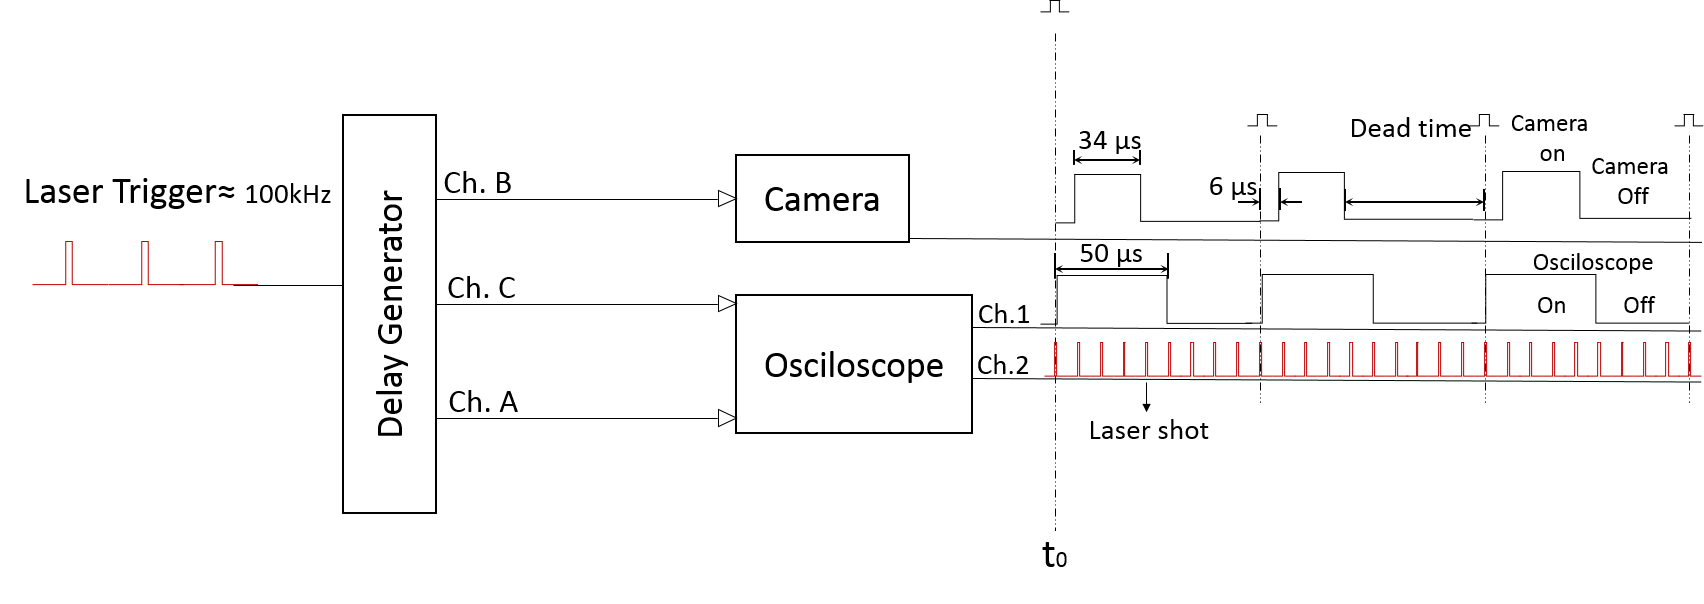
\includegraphics[width = 14 cm]{../Images/Trigger scheme.png}
\caption[Trigger Scheme]{Scheme of the trigger system used.  }
\end{figure}

In Fig \ref{fig:triggers}, we show the Trigger scheme used in the experiment. The oscilloscope and camera are triggered by the delayed channel B. The oscilloscope is set to $50\mu s$ and the camera to the minimal exposure time. So the camera and oscilloscope sees the same trigger, the oscilloscope will record at least 5 laser shots, but the camera because starts later just can see three as shown. The pictures are saved in the memory RAM of the computer so the dead time after the camera is off is mandatory to give the operating system enough time to save the data on disk and don't get out of ram. A small improvement in this system can be done if we trigger the camera with B and the oscilloscope with C, so both apparatus can start almost at the same time and no corrections need to be done. Each of the data set are saved with a unique label that will help to correlate the data after. Once an explosion is found in the VMI pictures, we check in its corresponding TOF that it has just one signal in all five laser shots, so we can be sure that picture correspond to a single coulomb explosion, in case more than one signal is found, this picture is discarded. 

\section{Calibration methods}
\subsection{VMI calibration}
To calibrate the VMI spectrometer,two different methods were used. A quadratic calibration function  $E=\alpha\cdot r^2$ is used, where $E$ is the kinetic energy of the particles and $r$ is the measured radius. This function is chosen because $E_{kin}=1/2 \cdot m v^2$. In order to keep simplicity,  stray fields, third order or linear terms are not included, as long as the calibration curves fit well with the measured.

On one hand, the most independant method is the trajectory simulation, because it does not rely on any lasersystem or physical process. Those simulations were made with SIMION 8.1. For the starting conditions for the electrons we chose a small interaction volume comparable to the estimated experimental conditions and the emission direction perpedicular to the spectrometer axis. For those electrons the projected energy on the detector screen is equivalent to the real kinetic energy, with this the inverse abel transformation can be avoided. It is neccessay to simulate different kinetic energies for the electrons, at different velocity vectors. After extracting the radii, where the electrons hit the detector plane, a calibration from pixels to mm for the camera is needed, because SIMION gives the radii of the electrons in mm. To do so, known distance in the camera image is needed, for example the inner diameter of the phosphor screen, making possible to generate the fit curve. The disadvantage of this method is, that it is very difficult to include any magnetic or electric stray fields into the simultions or other external parameter that can be in real.

\begin{figure}[h!]
\centering
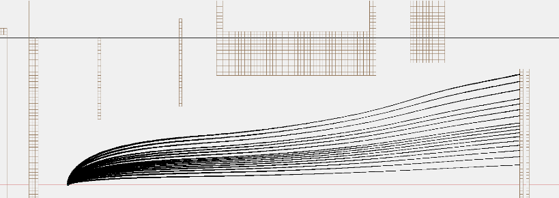
\includegraphics[scale=1]{../images/simion_calib.png}
\caption{energy calibration of the VMI spectrometer with SIMION. Electrons with discrete kinetic energy are emitted perpendicular to the spectrometer axis.}
\end{figure}


On the other hand, in order to contrast the simulation, a physical process is used, creating electrons with a well-known energy, then above threshold ionization (ATI) of raregas atoms is a suitable method to calibrate the spectrometer. The details about ATI of xenon can be found here xxx. The result of the ATI mechanism are several rings in the VMI along the laser polarization axis, that are energetically spaced by the energy of one photon. With at least 2 rings visible it is possible to do the calibration with the following formula
\begin{align*}
\Delta E = \alpha (r_2^2-r_1^2)
\end{align*}
where $\Delta E$ is the poton energy, $r_i$ are the peak positions of the abel inverted rings and $\alpha$ the calibration factor. Best results are achieved by using as low peak intensities as possible, so tunnel ionization is suppressed.

\begin{figure}[h!]
\centering
\includegraphics[scale=1]{../images/ati_calib.png}
\caption{energy calibration of the VMI spectrometer with the ATI method. The fringes are seperated by one photon energy, in this case 1.55eV}
\end{figure}

Another method to calibrate a VMI spectrometer is the use of a narrowband laser in combination with resonant processes. A very usefull scheme is published by \textit{Wituschek et al.} \cite{wituschek_simple_2016}. The scheme uses continuous 404nm laserlight to excite either the 5p${}_{3/2}$ or the 5p${}_{1/2}$ state in potassium. From this state, relaxation in four other states and the groundstate is possible. The 404nm light can also ionize electons from the resonant 5p state, the 5s, the 3d and the 4p states. The resulting electrons carry a very well defined kinetic energy $E_{kin}=E_{Photon}+E_{state}-E_{ionization}$. Since all energies on the right side of the equation are well known, the kinetic energy is also well known. This allows the calibration of the spectrometer with three points (the cross section of the 5s state is too small to see it) in the low energy range.

\begin{figure}
\centering
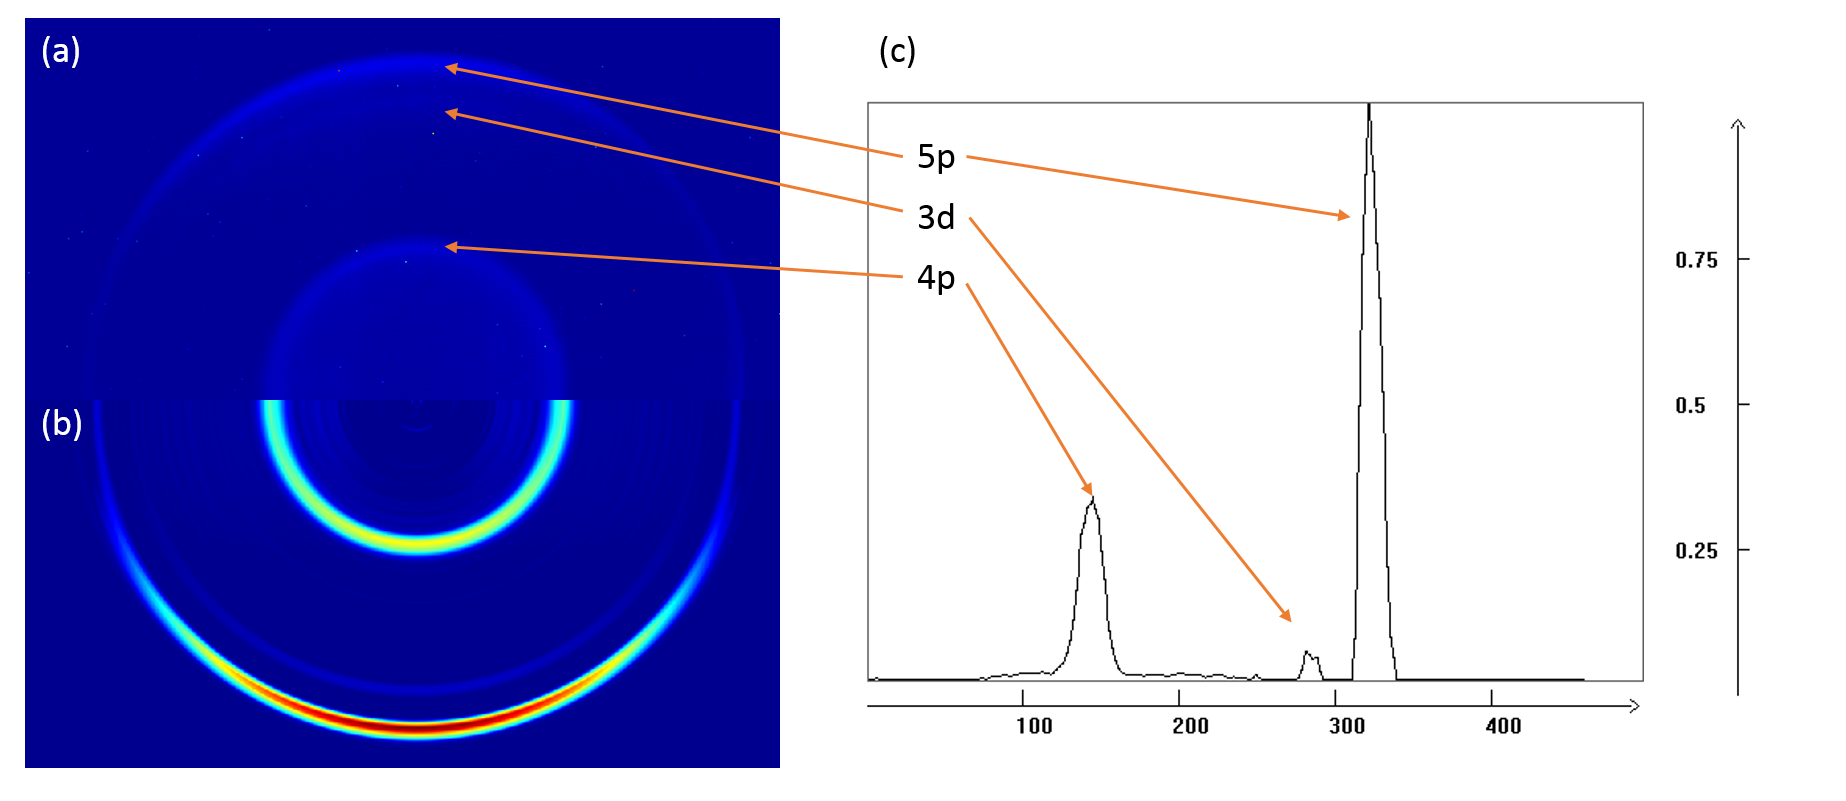
\includegraphics[scale=0.5]{../images/potassium_calib.png}
\caption{(a) Photoelectron image of potassium excited and ionized by linear polarized 404nm light, (b) abel inverted image and (c) corresponding photoelectron spectrum, not yet calibrated on the energy}
\end{figure}


\subsection{Laser intensity calibration}
When using a focused MIR and NIR laser, it is essential to know the peak intensity in the focus of the laserfield. Most of the time calculations give wrong results, because they assume a perfectly gaussian shape and do not account losses in optics after the power measurement or an inperfect focus. So it would be desirable to avoid caluclations and measure the peak intensity direclty. In this thesis two different schemes are used, the 2U$_P$ cutoff energy of electrons in a laserfield \cite{Becker_2018}, \cite{becker_vuv_1996} and the ratios of charge states of ions produced in the laser field \cite{augst_laser_1991}.




\section{Coulomb Explosion Model}
To explain the central feature in figure XXX a model for a coulomb explosion model from XXX is apllied. In this model a homogeniously charged sphere with radius $R$ is asumed and the charge distribution is given as a probability density function

\begin{align}
\frac{dP}{dr}=\frac{3 r^2}{R^3} \Theta (R-r)
\label{density_distribution}
\end{align}

where, $\frac{dP}{dr}$ is the probability to find an electron at radius $r$ and $\Theta$ is the Heavyside function. For this system the coulomb energy distribution $E_{coul}$ reads

\begin{align}
E_{coul}(r)=Ne^2 \frac{r^2}{R^3}
\label{coulomb_energy}
\end{align}

for $r\leq R$. $N$ is the number of electrons in the sphere and $e$ is the elementary charge of an electron. A charged sphere like this will immediately coulomb explode and for $t \longrightarrow \infty$ all coulomb energy is converted to kinetic energy, which can be measured experimentally with the VMI. It is possible to retrieve the energy distribution out of the spacial distribution \ref{density_distribution} with \ref{coulomb_energy} as the substitution formula.

\begin{align}
dr=\frac{R^3}{2Nq^2r}dE
\label{substitution}
\end{align}

Furthermore, we define the maximum coulomb energy

\begin{align}
E(R):=E_R=Nq^2 \frac{1}{R}
\label{max_coul_energy}
\end{align}

with all this follows the energy distribution of the electrons

\begin{align}
\frac{dP}{dE}=\frac{3}{2} \sqrt{\frac{1}{E_R}} \frac{1}{E_R}\sqrt{E} \cdot \Theta (1-\frac{E}{E_R})
\end{align}

it can be seen, that the energy distribution is fully characterized by $E_R$, so it is enough to know the maxium kinetic energy, which is just the radius of the central feature in our VMI images. With this even the inverse abel transformation can be bypassed, because the edge of a sphere in invariant for projecting the sphere on a plane.

With the formula for the homogenius density in a sphere

\begin{align}
R=(\frac{N}{\frac{4}{3} \pi \rho})^{1/3}
\end{align}

and formula \ref{max_coul_energy} the charge density in the beginning in the process can be derived to

\begin{align}
E_{max}(N)=\underbrace{\frac{e^2}{4 \pi \epsilon_0} (\frac{4}{3} \pi \rho)^{1/3}}_{=:B} N^{2/3}
\end{align}

and with this the charge density reads

\begin{align}
\rho=48 \pi^2 \frac{\epsilon_0^3}{e^6} B^3
\end{align}

In summary, the charge density can be calculated with the fit parameter $B$. $B$ can be retrieved by plotting the maximum kinetic energy $E_R$ as a function of the number of electrons $N$. Both can be extracted out of the VMI images, $E_R$ from the radius and $N$ from the brightness of the central feature.


\section{data analisis}
The High laser repetition rate compared to the Lor explsosion rate mentioned above, leads to a huge amoung of empty data. in oder wors , less than $10\%$ of all vmi pictures and TOF spectra didn conain any nanoplasma explosion. So a signal finder procesing, in mathematica software, was impplemented. In the next section we will explain the signal recognition algorithms and the data processing, as well as the first assumption of our model to explaing the threatment given to the results. 
\subsection{Event recognision}

As mentioned, the low event rate of nano plasma explosions results in a lot of emtpy VMI images. In average 10000 pictures where taken for each set of data where, less than $7\%$ of them contain signal, in the best  systems. A typical VMI signal can be seen in fig \ref{fig:vmiexample}, where regarding if its NIR or MIR, a central feature with circular distribution is presented. However, the angular an radial distribution changes, depending of the experiment. When the uncoupled mode of the spectrometers is used, like in the NIR measurements, the VMI images have to be sorted without the help of the TOF traces.

To seperate empty images from images with events the central feature is used. A center is selected manually and all pixels within a region around the center are summed up. If the sum is above a certain threshold value the image contains a signal. To analyze the central feature in more detail the size and the brightness of this feature is of importance. To determine the radius and the brightness, two methods were compared, one using the mathematica 10.1 (wolfram inc.) algorithm and the other using a bining processing., both explained on next.

First, the ImageMeasurements and Componentmeasurements  algoriths in mathematica act, over binnirized images, works with arbitrary 2D and 3D images and computes  multiple porperties, finding components bases on an specifc matrix. For this special case, a circular matrix with specifications of minimun radius and  no share edges were given as paramneters. The efficient of this process was demostrared to depent stronglly on the initial image and the signal-noise rate, hence, a recursive funtion when develop to change the binarized threshold  recursively until the algprithm find just one object that matchs the signal. The thrshold was changed progresively and modifyable steps in order to get the most precise fit. Once the object is found, the radius and center are save, and sum the total intensity inside the radius, so a radius-Brigthness  meassument ius compleat for each invividual image.

The secon method was based on a circula binning of the signal. A center for each data set is manually place afte summed all signal pictures and find the center of the signal blop, set to be at the same position within one measurement. Three circles are defined around this center, the first one with radius $r$ (in pixels), which is variale, the second one with $r_{in} = r-\Delta r$ and the last one with $r_{out} = r + \Delta r$, where $\Delta r$ has to be picked out from the dataset. The three circles define two areas $A_{in}$ and $A_{out}$, see figure XXX. An average pixelvalue $\rho$ for both areas is defined via

\begin{align}
\rho_{in} & = \frac{1}{N_{in}} \sum_{px \in A_{in}} \text{value}(px) \\
\rho_{out} & = \frac{1}{N_{out}} \sum_{px \in A_{out}} \text{value} (px)
\end{align}

where $N$ is the number of pixels in the respective area. The normalization on the area is important, because the areas are of different size. To finally find out the radius of the central blop, the difference $\rho_{in}-\rho_{in}$ is maximized, this is the case for the orange box in figure XXX. For the green and the purple boxes $\rho_{in} = \rho_{in}$, which gives zero for the difference.
Real signals do not have a perfect cutoff or a constant radial profile, which leads to noisy curves, when $\Delta r$ is chosen too small, which makes the determination of $r$ difficult. An example for a single shot image, where the radius is determined for $\Delta r = 3,4,5$ in pixels, is shown in figure \ref{fig:density_plot}. The VMI image in this figure has a donut shape, if the inner radius is of interest the same curve can be used to determine the inner radius as well if the minimum of the function is taken.

\begin{figure}

\centering
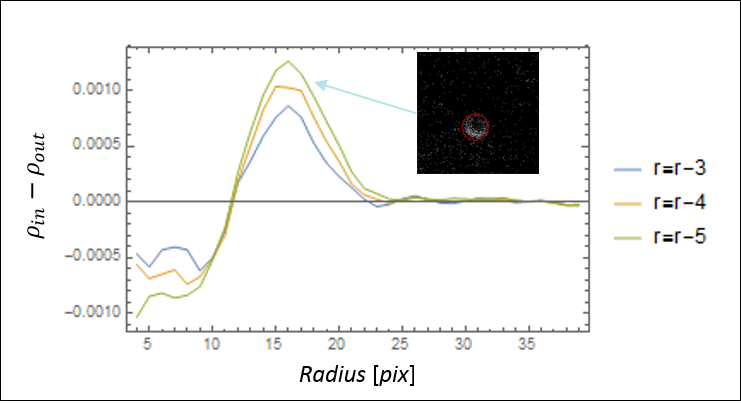
\includegraphics[width=10 cm]{../images/density_plot.png}
\caption{Difference of mean pixel values to determine the radius of the central feature in the VMI images}
\label{fig:density_plot}
\end{figure}
As shown in \ref{fig:density_plot}, the density difference have a sumit in tho cases, one when the inner our outer density changes signs. The lower peak, when exists, reffers to the change from a low density change to a high one, besides the higher peak, describe the change from a high desnsity to a lower, setting the radius where the edge of the blop is. pointing out that not all signals have the donut shape so this case was just added when needed. Finally, as in the last procedure, the inner pixels in the circle with radius $r$ are summed and the radius-Brigthnes is save for all signal. In the case, as the example, where the second inner circle is clearly identified, the sum of all the pixel discard the inner are, and at the same time, adds the inner radius-brightness measurements to it. 
Both radius finder functions where always double checked by taking random signal images and highlighting the radius found. Figure \ref{fig:checkradius} shows a set of well fitted radius for each signal, proving the good efficiency of the algorithms. 

\begin{figure}[hbtp]
\caption{Example of ramdom signal images fitted to ir corresponding radius.}
\centering
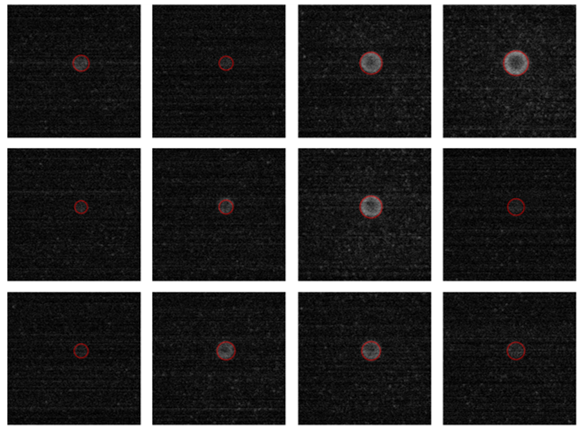
\includegraphics[width=10cm]{../Images/density_plot_chekc.png}
\label{fig:checkradius}
\end{figure}
Last, once the radius-brightness data is recorded, and the calibrations are set, the system can be compare to the model explained above, where radius can be converted itio maximal kinetic energy, $r\rightarrow k_{energy}$, and brightness to number of electrons, $b\rightarrow N_{e-}$. 

